\subsection{Leisungsbudget}
Somit lagen bereits einige Kennzahlen vor, die eingehalten werden mussten:
\paragraph{Anzahl Exciter: 6} Dies ist durch den Korpusaufbau gegeben. Eine höhere Anzahl hätte zwar akustisch einige Vorteile, ist aber mit grösseren Dimensionen und/oder höheren Kosten verbunden.
\paragraph{Leistung (RMS) pro Exciter: 0.5 bis 150 Watt} Dies sind zunächst der Bereich der Leistungskennzahlen aller verfügbaren Exciter auf \href{https://www.soundimports.eu/en/audio-components/exciters/?hr-page=%7B%22page%22%3A1%2C%22active_filter%22%3A%22%22%2C%22filters%22%3A%5B%5D%2C%22product_count%22%3A0%7D}{soundimports.eu}. Da solche Exciter oft für Kino-Effekte wie z.B. Vibrationen des Tyrannosaurus Rex verwendet werden, gibt es entsprechend Modelle für Bassfrequenzen mit Leistungsangaben bis 150W. Da bei dieser Arbeit das Ziel einer möglichst tiefen Grenzfrequenz nicht im Vordergrund stand (siehe \nameref{sec:zielgewichtung}), kamen wesentlich kleinere Modelle für die Exciter in Frage. Zu den Leistungskennzahlen allerdings noch ein kurzer Einschub, da diese immer wieder zu Missverständnissen führen:
\subsubsection{Leistungsangaben bei Lautsprechern} \label{chap:leistungsangaben} In der Audioindustrie werden in der Regel mindestens drei Kennzahlen für die Maximalleistung eines Lautsprechers genannt:
\begin{itemize}
	\item \textbf{RMS Power Handling} oder auch \textbf{Power Cont.} oder auch \textbf{Rated Noise Power}
	\item \textbf{Power(Programm)} oder auch \textbf{Rated Power}
	\item \textbf{Peak Power} oder auch \textbf{Power handling Peak}
\end{itemize}
Diese Begriffe werden teilweise sehr unterschiedlich verwendet, bisweilen auch vom selben Hersteller. Es ist am einfachsten, beim letzten Begriff zu beginnen:
\textbf{Peak Power} beschreibt die absolut maximale Leistung, die ein Lautsprecher zu einem einzelnen Zeitpunkt noch verträgt. Also führt einem Signal mit einem 1mW höheren Spitzenwert (theoretisch) zur Zerstörung des Produkts.
Der Peak-Wert wird nun als Ausgangsbasis verwendet, um den Effektivwert (RMS) der Leistung zu berechnen. Dieser hängt allerdings stark vom Crest-Faktor, also dem Verhältnis zwischen Spitzen- und Effektivwert eines Signals, ab. Die \citetitle{aespar} der Acoustic Engineering Society (AES)  erläutert den Begriff:
\begin{quotation}
	\textbf{crest factor} The term used to represent the ratio of the peak (crest) value to the rms value of a waveform measured over a specified time interval. For example, a sine wave has a crest factor of 1.4 (or 3 dB), since the peak value equals 1.414 times the rms value. Music has a wide crest factor range of 4-10 (or 12-20 dB) [\textit{Hier wird in Volt, also 6dB pro Verdopplung gerechnet.}]. This means that music peaks occur 12-20 dB higher than the rms value, which is why headroom is so important in audio design.\\Quelle: \cite{aespar} \label{cite:crest}
\end{quotation}
%\begin{quotation}
%	As we've mentioned, pink noise can have various crest factors, but the crest factor in testing is typically 2 [\textit{Spannungsbezogen}].\\Quelle: \cite{SoundreinforcementforaudioEngineers}
%\end{quotation}
In der Praxis wird also ein Testsignal\footnote{gemäss IEC 60268-1:1985} verwendet, welches typischerweise einen Crest-Faktor von 6dB (Leistungsbezogen) hat. Somit ist der Wert für \textit{RMS Power Handling} oder \textit{Cont. Noise Power} 4-mal tiefer als der Peak Wert.
Da Lautsprecher immer von Endstufen getrieben werden, muss diese nun auch die Leistung des Lautsprechers liefern können. Andernfalls wird die in vielen Endstufen vorhandene Leistungsbegrenzung (eng. \textit{Limiter}) aktiviert und somit ein Gleichspannungssignal mit Vollausschlag erzeugt, welches die Schwingspule im Lautsprecher maximal stark auf eine Seite hin auslenkt und somit den Lautsprecher beschädigen oder gar zerstören kann. Die Endstufe muss also mindestens die nominale RMS-Leistung des Lautsprechers liefern können. In der Praxis wird hier als Nominalwert für die Endstufe die doppelte RMS-Leistung des Lautsprechers empfohlen, damit die Endstufe auch alle Signalspitzen gut abbilden kann. Durch digitale Limiter-Presets, welche Grenzwerte für RMS und Peak enthalten, kann der Schutz des Lautsprechers sichergestellt werden. 
Abbildung \ref{pics:adc820_pwr} zeigt diese Angaben aus einem Datenblatt eines Deckeneinbaulautsprechers (\cite{adc820man}). Jedoch wird keine Peak-Leistung angegeben. Abbildung \ref{pics:adc820_footnote} zeigt die Fussnoten, welche einen Crestfaktor von 6dB angeben.
\begin{figure}[H]
	\centering
	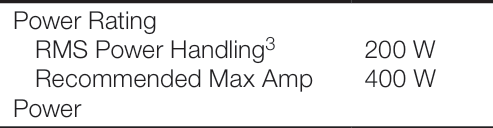
\includegraphics[width=\textwidth*5/9]{pictures/adc820_pwr.png}
	\caption{Leistungsangaben eines Deckenlautsprechers, ohne Peak Power}
	\label{pics:adc820_pwr}
\end{figure}
\begin{figure}[H]
	\centering
	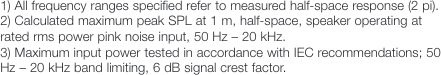
\includegraphics[width=\textwidth*5/9]{pictures/adc820_footnotes.png}
	\caption{In den Fussnoten findet sich der Crest-Faktor}
	\label{pics:adc820_footnote}
\end{figure}
\subsubsection{Entscheid Exciterleistung}
Aus den Vorarbeiten ging heraus, dass bereits ein Excitermodell mit 10W RMS-Leistung extrem Effizient und weitaus höhere Schallpegel erzeugt als in dieser Anwendung erfordert. Der dabei verwendete Exciter war ein \textbf{DAEX25QLP-4} von Dayton Audio. Abbildung \ref{pics:DAEX25QLP4_freqresp} zeigt den Frequenzgang dieses Modells. Dieser bewegt sich durchschnittlich im Bereich von 75-80 dB SPL\footnote{Eine SPL-Nominalwert wird im Datenblatt nicht angegeben. Zudem fehlt die Angabe ob A-, B- oder Z-Gewichtet wurde}. Der Vergleich mit dem kleineren Modell \textbf{DAEX19QLP-4} (Abbildung \ref{pics:DAEX19QLP4_freqresp}) zeigt, dass dieser im Bereich von 100-1000Hz zwar ca. 5 dB weniger Pegel erzeugt, darüber sogar noch einen lineareren Frequenzgang aufweist. Aus dieser Beobachtung wurde geschlossen, dass auch ein \textbf{Exciter mit 5W RMS} bereits für diese Anwendung ausreicht. Aus Zeitgründen und um genug Headroom für hohe Signalpegel zu haben, wurde darauf verzichtet, noch kleinere Leistungsmodelle zu evaluieren.
\begin{figure}[H]
	\centering
	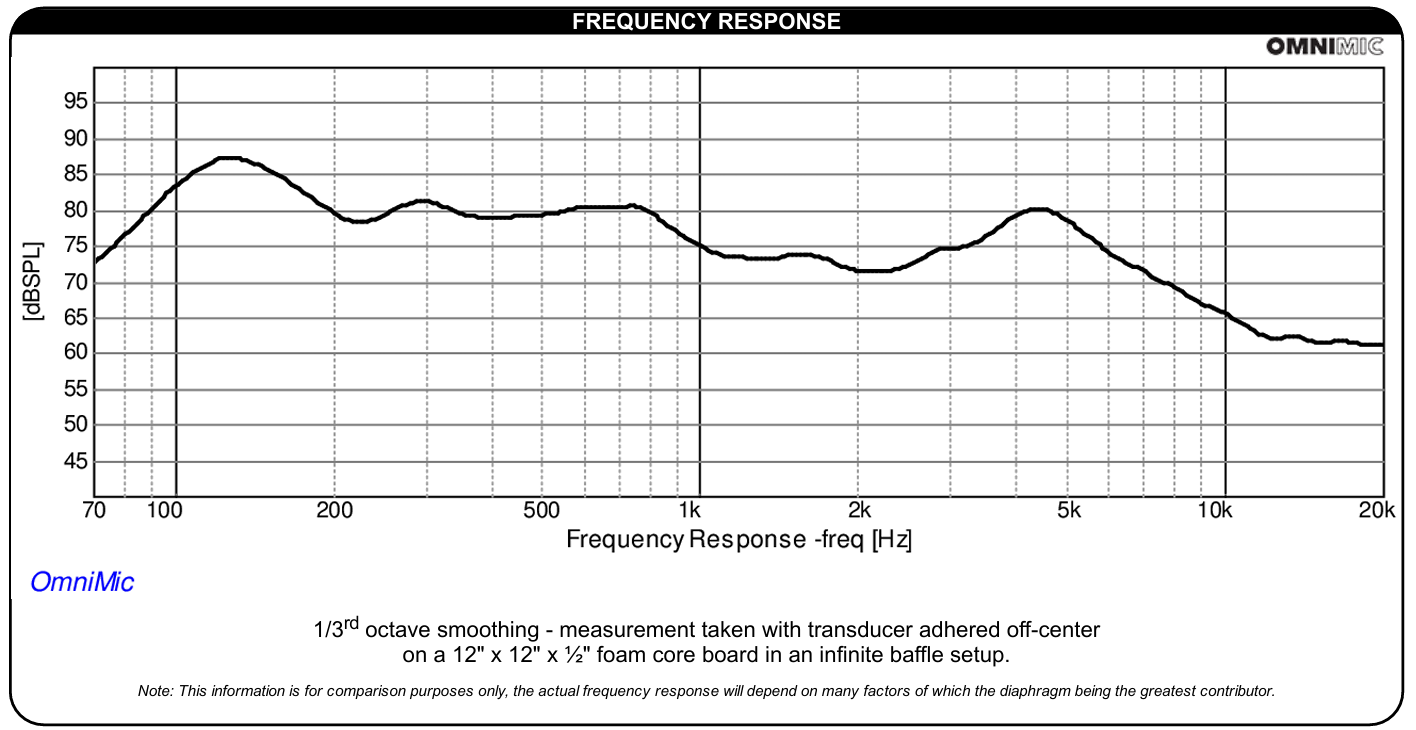
\includegraphics[width=\textwidth*7/8]{pictures/DAEX25QLP4_freqresp.png}
	\caption{Quelle: \cite{DAEX25QLP4spec}}
	\label{pics:DAEX25QLP4_freqresp}
\end{figure}
\begin{figure}[H]
	\centering
	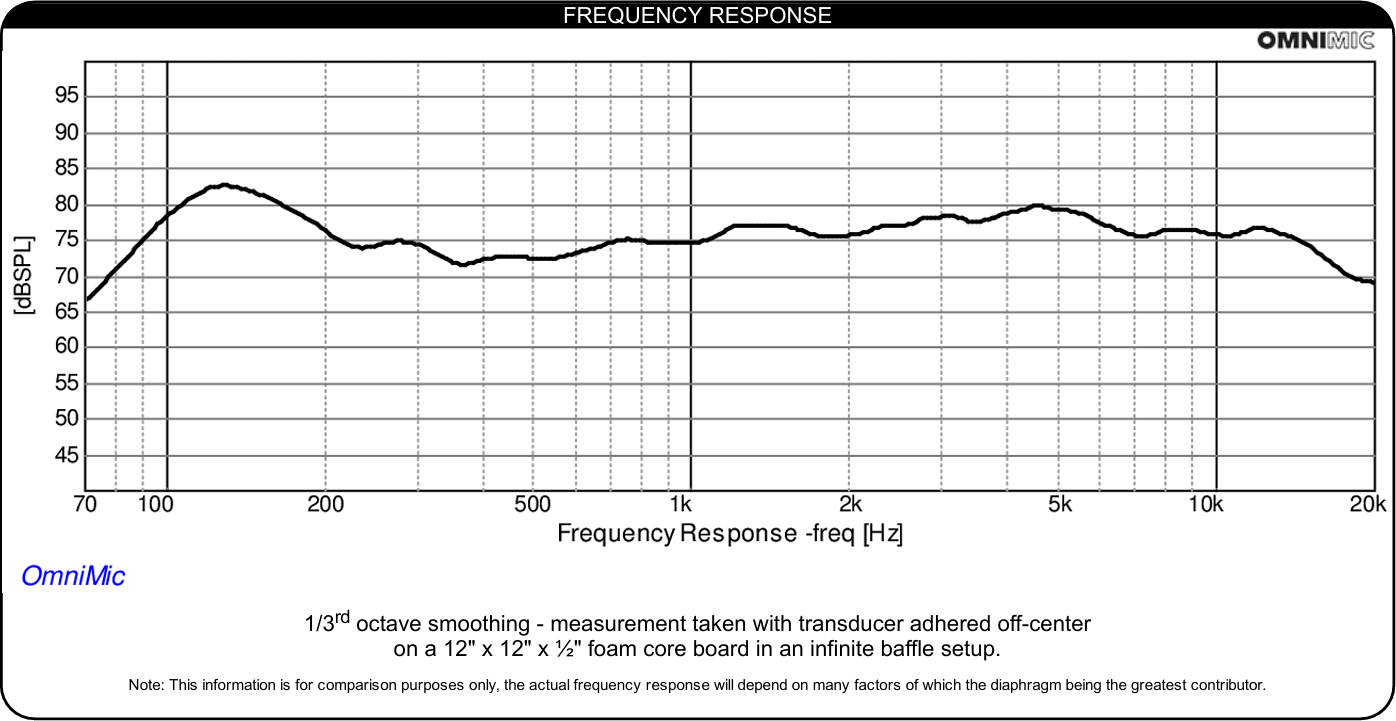
\includegraphics[width=\textwidth*7/8]{pictures/DAEX19QLP4_freqresp.png}
	\caption{Quelle: \cite{DAEX19QLP4spec}}
	\label{pics:DAEX19QLP4_freqresp}
\end{figure}
\subsubsection{PoE}
In der Netzwerktechnik als weit verbreiteter Standard zur gleichzeitigen Übertragung von Speisung und Daten etabliert, bietet PoE (\textit{Power over Ethernet}) eine extrem einfache und Attraktive Lösung für dieses Projekt. Jedoch hat der Standard auch einige Tücken, und gerade die höheren Leistungsklassen (PoE++) können schnell extrem kostenintensiv werden. Zudem hängt das ganze nochmals vom verwendeten Kabel, und dessen Querschnitt ab. Abbildung \ref{pic:poe_overview} zeigt eine anschauliche Übersicht über den Standard und die verfügbaren Leistungen (Quelle: \cite{PoE_overview_doc}).
\begin{figure}[H]
	\centering
	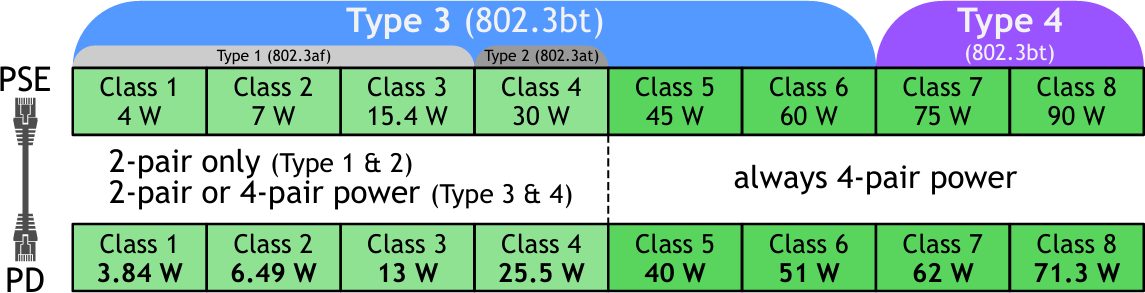
\includegraphics[width=\textwidth*3/4]{pictures/PoE_overview.png}
	\caption{Eine Übersicht über die PoE-Klassen}
	\label{pic:poe_overview}
\end{figure}
\subsubsection{Gesamtes Leisungsbudget}
Mit dem Wissen aus \ref{chap:leistungsangaben} kann nun eine Aussage über die voraussichtlich benötigte Nominalleistung der Endstufe und der Speisung gemacht werden. {\color{red} Zu beachten ist, dass das MILAN-Modul direkt durch PoE gespiesen wird und somit in der Leistungsberechnung entfällt.} In einer Grafik können nun alle Leistungswerte Eingetragen werden (Abbildung \ref{pic:Leistungsbudget}). Darin sind zum Vergleich auch die am Gerät verfügbaren Nennleistungen der PoE-Klassen (PoE, PoE+ und PoE++). Es zeigt sich somit, dass auch die höchste PoE-Klasse nur sehr knapp die geforderte Leistung zu erbringen vermag (bzw. nur mit einem sehr aufwändigem Puffer) und daher als alleinige Speisung für das komplette Gerät nicht infrage kommt.
\begin{figure}[H]
	\centering
	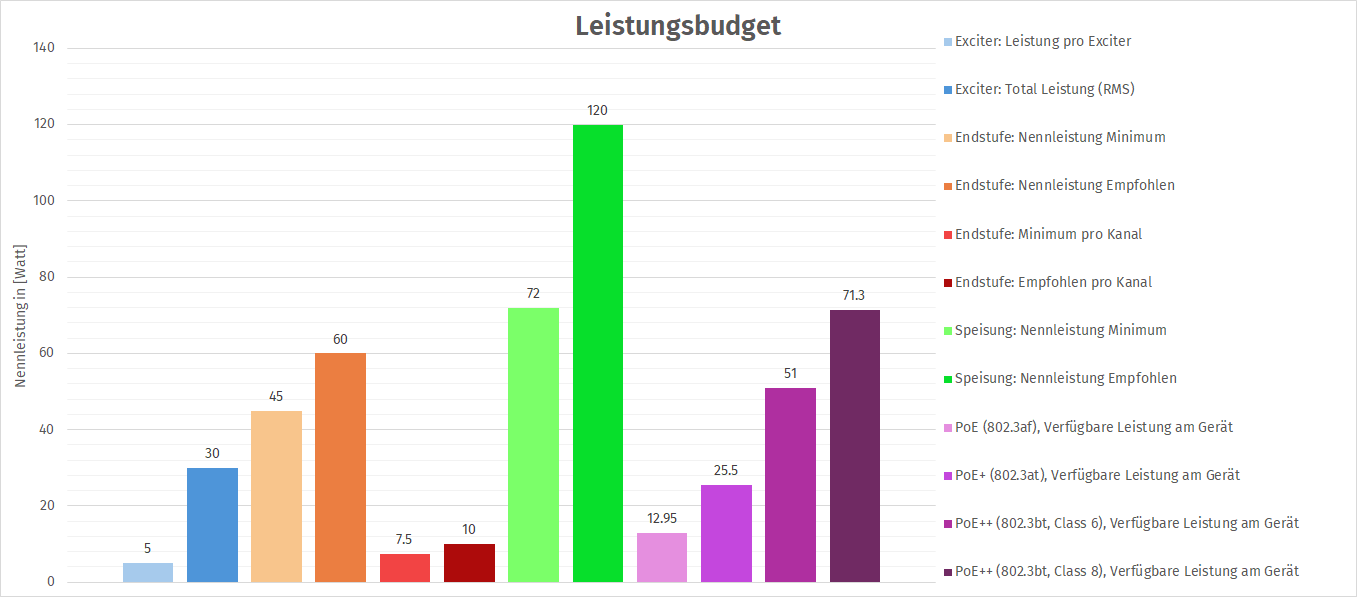
\includegraphics[width=\textwidth]{pictures/Leistungsbudget.png}
	\caption{Das Leistungsbudget}
	\label{pic:Leistungsbudget}
\end{figure}
